% move all configuration stuff into one file so we can focus on the content
\documentclass[aspectratio=169,hyperref={pdfpagelabels=false,colorlinks=true,linkcolor=white,urlcolor=blue},t]{beamer}

%%%%%%%%%%%%%%%%%%%%%%%%%%%%%%%%%%%%%%%%%%%%%%%%%%%%%%%%%%%%%%%%%%%%%%%%%%%%%%%%%%
%%%%%%%%%%%%%%%%%%%%%%%%%%%%%%%%%%%%%%%%%%%%%%%%%%%%%%%%%%%%%%%%%%%%%%%%%%%%%%%%%%
% packages
\usepackage{pict2e}
\usepackage{epic}
\usepackage{amsmath,amsfonts,amssymb}
\usepackage{units}
\usepackage{fancybox}
\usepackage[absolute,overlay]{textpos} 
\usepackage{media9} % avi2flv: "C:\Program Files\ffmpeg\bin\ffmpeg.exe" -i TuneFreqFilterbank.avi -b 600k -s 441x324 -r 15 -acodec copy TuneFreqFilterbank.flv
\usepackage{animate}
\usepackage{gensymb}
\usepackage{multirow}
\usepackage{silence}
\usepackage[backend=bibtex,style=ieee]{biblatex}
\AtEveryCitekey{\iffootnote{\tiny}{}}
\addbibresource{references}

%%%%%%%%%%%%%%%%%%%%%%%%%%%%%%%%%%%%%%%%%%%%%%%%%%%%%%%%%%%%%%%%%%%%%%%%%%%%%%%%%%
%%%%%%%%%%%%%%%%%%%%%%%%%%%%%%%%%%%%%%%%%%%%%%%%%%%%%%%%%%%%%%%%%%%%%%%%%%%%%%%%%%
% relative paths
\graphicspath{{graph/}}


%%%%%%%%%%%%%%%%%%%%%%%%%%%%%%%%%%%%%%%%%%%%%%%%%%%%%%%%%%%%%%%%%%%%%%%%%%%%%%%%%%
%%%%%%%%%%%%%%%%%%%%%%%%%%%%%%%%%%%%%%%%%%%%%%%%%%%%%%%%%%%%%%%%%%%%%%%%%%%%%%%%%%
% units
\setlength{\unitlength}{1mm}

%%%%%%%%%%%%%%%%%%%%%%%%%%%%%%%%%%%%%%%%%%%%%%%%%%%%%%%%%%%%%%%%%%%%%%%%%%%%%%%%%%
%%%%%%%%%%%%%%%%%%%%%%%%%%%%%%%%%%%%%%%%%%%%%%%%%%%%%%%%%%%%%%%%%%%%%%%%%%%%%%%%%%
% theme & layout
\usetheme{Frankfurt}
\beamertemplatenavigationsymbolsempty
%\setbeamertemplate{frametitle}[smoothbars theme]
\setbeamertemplate{frametitle}
{
    \begin{beamercolorbox}[ht=1.8em,wd=\paperwidth]{frametitle}
        \vspace{-.1em}%
        \hspace{.2em}{\strut\insertframetitle\strut}
        
        \hspace{.2em}\small\strut\insertframesubtitle\strut
        %\hfill
        %
\includegraphics[height=.8cm,keepaspectratio]{CenterMusicTechnology-solid-2lines-white-CoAtag}
        
    \end{beamercolorbox}
    \begin{textblock*}{100mm}(11.6cm,.7cm)
        \includegraphics[height=.8cm,keepaspectratio]{logo_GTCMT_black}
    \end{textblock*}
}

% set this to ensure bulletpoints without subsections
\usepackage{remreset}
\makeatletter
\@removefromreset{subsection}{section}
\makeatother
\setcounter{subsection}{1}

%---------------------------------------------------------------------------------
% appearance
\setbeamercolor{structure}{fg=gtgold}
\setbeamercovered{transparent} %invisible
\setbeamercolor{bibliography entry author}{fg=black}
\setbeamercolor*{bibliography entry title}{fg=black}
\setbeamercolor*{bibliography entry note}{fg=black}

%\usepackage{pgfpages}
%\setbeameroption{show notes}
%\setbeameroption{show notes on second screen=right}
%---------------------------------------------------------------------------------
% fontsize
\let\Tiny=\tiny

%%%%%%%%%%%%%%%%%%%%%%%%%%%%%%%%%%%%%%%%%%%%%%%%%%%%%%%%%%%%%%%%%%%%%%%%%%%%%%%%%%
%%%%%%%%%%%%%%%%%%%%%%%%%%%%%%%%%%%%%%%%%%%%%%%%%%%%%%%%%%%%%%%%%%%%%%%%%%%%%%%%%%
% warnings
\pdfsuppresswarningpagegroup=1
\WarningFilter{biblatex}{Patching footnotes failed}
\WarningFilter{latexfont}{Font shape}
\WarningFilter{latexfont}{Some font shapes}
\WarningFilter{gensymb}{Not defining}



\subtitle{Part 4.3: Feature Post-Processing}

%%%%%%%%%%%%%%%%%%%%%%%%%%%%%%%%%%%%%%%%%%%%%%%%%%%%%%%%%%%%%%%%%%%%%%%%%%%%
\begin{document}
    % generate title page
	

\begin{frame}
    \titlepage
    %\vspace{-5mm}
    \begin{flushright}
        \href{http://www.gtcmt.gatech.edu}{\includegraphics[height=.8cm,keepaspectratio]{logo_GTCMT_black}}
    \end{flushright}
\end{frame}


    \section[overview]{lecture overview}
        \begin{frame}{instantaneous features}{overview}
            \begin{itemize}
                \item   \textbf{text book}  
                    \begin{itemize}
                        \item   \href{http://ieeexplore.ieee.org/xpl/articleDetails.jsp?tp=&arnumber=6331121&}{\underline{\textit{Chapter 4: Intensity} (pp.~71--78)}}
                    \end{itemize}
                \bigskip
                \item<2->   \textbf{lecture content}
                    \begin{itemize}
                        \item<2->   
                        \item<3->   
                        \item<4->   
                    \end{itemize}
            \end{itemize}
        \end{frame}

    \section[intro]{introduction}

        \begin{frame}{intensity, magnitude \& loudness}{introduction}
            \begin{itemize}
                \item   intensity-related descriptors \textbf{commonly used}
                    \begin{itemize}
                        \item	waveform view
                        
                            \includegraphics[scale=.3]{waveforms}
                        \item	level monitoring (PPM, VU,\ldots)
                        
                            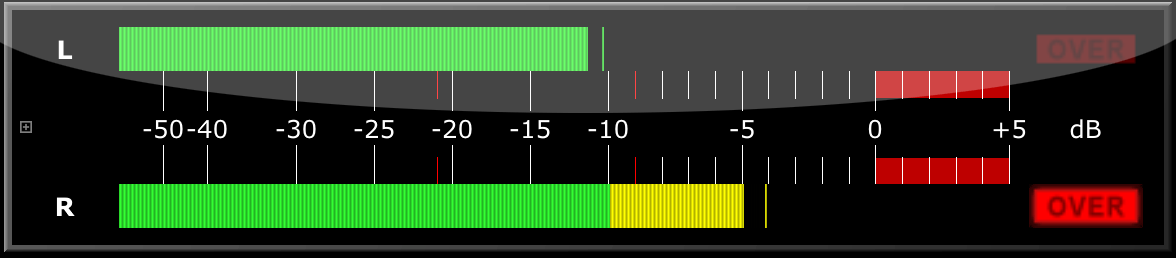
\includegraphics[scale=.1]{ppmulator}
                     \end{itemize}
            \end{itemize}
            
            \vspace{-3mm}
            \begin{itemize}
                \item[]<2-> \question{terms and definitions}
                \vspace{-3mm}
                 \begin{itemize}
                    \item	intensity
                    \item	magnitude
                    \item	peak
                    \item	envelope
                    \item	level
                    \item	volume
                    \item	loudness
                 \end{itemize}
            \end{itemize}
            
                \vspace{-3mm}
        \end{frame}
	
	\begin{frame}{intensity, magnitude \& loudness}{human perception 1/2}
		perception has non-linear relation to intensity:
		\begin{itemize}
			\item	model: logarithmic relation
				\begin{equation}
					v_\mathrm{dB}(n) = 20\cdot\log_{10}\left(\frac{v(n)}{v_0}\right)
				\end{equation}
	
				\pause
				\begin{itemize}
					\item	$v_0$: reference constant (\unit[0]{dB} point)
					
							digital: $v_0 = 1$ $\Rightarrow \unit{dBFS}$
					\pause
					\item	scaling	factor: \unit[1]{dB} $\approx$ JNDL
				\end{itemize}
		\end{itemize}
	\end{frame}
	
	%\begin{frame}{intensity, magnitude \& loudness}{comment: level computation}
		%$v(n) = 0$: computation of $\log_{10}(0)$
		%
		%workarounds:
		%\begin{itemize}
			%\item	add constant $\epsilon$
				%\begin{equation}
					%v_\mathrm{dB}(n) = 20\cdot\log_{10}(v(n) + \epsilon)
				%\end{equation}
				%\begin{figure}
					%\centering
						%\includegraphics[scale=.7]{\AcaGraph/logepsilon}
					%\label{fig:logepsilon}
				%\end{figure}
				%
			%\pause
			%\item	add \textbf{if} statement	
				%\begin{equation}
					%v_\mathrm{trunc}(n)  =   \left\{ 
								%\begin{array}{ll} 
									%v(n), & \text{if } v(n) \geq \epsilon \\
									%\epsilon, & \text{otherwise }
			          			%\end{array} 
			          			%\right. 
				%\end{equation}
		%\end{itemize}
	%\end{frame}
	%
	%\begin{frame}{intensity, magnitude \& loudness}{human perception 2/2}
		%decibel scale is \textit{not} loudness scale:
		%\begin{itemize}
			%\item	equal-sized steps on the decibel scale not perceived as equal-sized loudness steps
		%\end{itemize}
		%
		%\pause
		%\bigskip
		%perceptual loudness depends on
		%\begin{itemize}
			%\item	frequency
			%\item	cochlear resolution
			%\item	masking effects
		%\end{itemize}
		%\vspace{-20mm}
		%\begin{figure}
			%\flushright
				%\includegraphics[scale=.25]{graph/equalloudness}
		%\end{figure}
	%\end{frame}	
	%
	%\begin{frame}{intensity, magnitude \& loudness}{dynamics in music}
		%\begin{itemize}
			%\item	\textbf{score}:
					%\begin{itemize}
						%\item	only several rough dynamic steps,e.g., \emph{\textbf{pp}}, \emph{\textbf{p}}, \emph{\textbf{mf}}, \emph{\textbf{f}}, \emph{\textbf{ff}}
						%\item	comparably vague instructions on volume modifications, e.g., \textsl{crescendo}, \textsl{decrescendo}, \emph{\textbf{sf}}
						%\pause
						%\item	dynamics influenced by
								%\begin{itemize}
									%\item	instrumentation
									%\item	timbre
									%\item	number of voices
									%\item	context and musical tension
								%\end{itemize}
					%\end{itemize}
			%\item	\textbf{MIDI}:
					%\begin{itemize}
						%\item	$128$ velocity steps
						%\item	no standardized relation to magnitude, power, \ldots
					%\end{itemize}
		%\end{itemize}
	%\end{frame}
	%\begin{frame}{intensity, magnitude \& loudness}{features: root mean square 1/2}
		%\begin{equation}\label{eq:rms}
			%\input{\AcaEq/Llf_RMS}
		%\end{equation}
			%\begin{figure}
				%\includegraphics[scale=.7]{\AcaGraph/rms}
			%\end{figure}
	%\end{frame}
	%\begin{frame}{intensity, magnitude \& loudness}{features: root mean square 2/2}
			%\begin{itemize}
				%\item	measure of power
			%\end{itemize}
			%
			%\pause
			%\textbf{variants}  (sample processing only):
			%\begin{itemize}
				%\item	reduce computational complexity
					%\begin{footnotesize}
					%\begin{eqnarray}
						%v^2_{\mathrm{RMS}}(n) &=& \frac{x(i_{\mathrm{e}}(n))^2 - x(i_{\mathrm{s}}(n-1))^2}{i_{\mathrm{e}}(n)-i_{\mathrm{s}}(n) + 1} + v^2_{\mathrm{RMS}}(n-1) \\
						%v_{\mathrm{RMS}}(n)	&=& \sqrt{v^2_{\mathrm{RMS}}(n)}
					%\end{eqnarray}
					%\end{footnotesize}
				%\item	single pole approximation
					%\begin{footnotesize}
					%\begin{eqnarray}
						%v_\mathrm{tmp}(i)	&=& \alpha\cdot v_\mathrm{tmp}(i-1) + (1-\alpha)\cdot x(i)^2\\
						%v^*_{\mathrm{RMS}}(i)		&=& \sqrt{v_\mathrm{tmp}(i)}
					%\end{eqnarray}
					%\end{footnotesize}
			%\end{itemize}
	%\end{frame}
	%\begin{frame}{intensity, magnitude \& loudness}{features: weighted root mean square}
		%\vspace{-5mm}
		%\begin{figure}
			%\centering
			%\begin{footnotesize}
	\setcounter{iXOffset}{0}
	\setcounter{iYOffset}{5}
	\setcounter{iXBlockSize}{20}
	\setcounter{iYBlockSize}{16}
	\setcounter{iDistance}{5}
	\setcounter{iYBlockSizeDiv2}{8}
    \begin{picture}(57,26)


		\addtocounter{iYOffset}{\value{iYBlockSizeDiv2}}
		\addtocounter{iYOffset}{1}
        \put(\value{iXOffset},\value{iYOffset}){\footnotesize{\shortstack[c]{$x(i)$}}}
		\addtocounter{iYOffset}{-1}
		\addtocounter{iXOffset}{2}

        \put(\value{iXOffset},\value{iYOffset}){\vector(1,0){\value{iDistance}}}
		\addtocounter{iYOffset}{-\value{iYBlockSizeDiv2}}

		\addtocounter{iXOffset}{\value{iDistance}}
        \put(\value{iXOffset},\value{iYOffset}){\framebox(\value{iXBlockSize}, \value{iYBlockSize}){\footnotesize{\shortstack[c]{$H(z)$}}}}

		\addtocounter{iXOffset}{\value{iXBlockSize}}
		\addtocounter{iYOffset}{\value{iYBlockSizeDiv2}}
        \put(\value{iXOffset},\value{iYOffset}){\vector(1,0){\value{iDistance}}}
		\addtocounter{iYOffset}{-\value{iYBlockSizeDiv2}}

		\addtocounter{iXOffset}{\value{iDistance}}
        \put(\value{iXOffset},\value{iYOffset}){\framebox(\value{iXBlockSize}, \value{iYBlockSize}){\footnotesize{\shortstack[c]{$\mathrm{RMS}$}}}}

		\addtocounter{iXOffset}{\value{iXBlockSize}}
		\addtocounter{iYOffset}{\value{iYBlockSizeDiv2}}
        \put(\value{iXOffset},\value{iYOffset}){\vector(1,0){\value{iDistance}}}

        %text
		\addtocounter{iYOffset}{1}
		\addtocounter{iXOffset}{3}
        \put(\value{iXOffset},\value{iYOffset}){\footnotesize{\shortstack[c]{$v(n)$}}}

    \end{picture}
\end{footnotesize}

	    %\end{figure}
	    %
	    %\pause
		%\vspace{-10mm}
	    %$H(z)$:
	    %\begin{itemize}
	    	%\item	A, B, C weighting
	    	%\item	RLB (BS.1770)
	    	%\item	\ldots
	    %\end{itemize}
	    %
		%\begin{figure}
			%\centering
			%\includegraphics[scale=.7]{\AcaGraph/loudnessweighting}
			%\label{fig:loudnessweighting}
		%\end{figure}
	%\end{frame}
	%\begin{frame}{intensity, magnitude \& loudness}{features: peak envelope (max)}
		%\begin{equation}
			%v_{\mathrm{Peak}}(n) = \max_{i_{\mathrm{s}}(n) \leq i \leq i_{\mathrm{e}}(n)}{|x(i)|} 
		%\end{equation}
		%\begin{figure}
			%\centering
				%\includegraphics[scale=.7]{\AcaGraph/ppm}
		%\end{figure}
	%\end{frame}
	%\begin{frame}{intensity, magnitude \& loudness}{features: peak envelope (PPM) 1/2}
		%\begin{figure}
			%\centering
			%				\begin{footnotesize}
					\begin{picture}(100,40)(0,0)
			
						\put(-0.5,30){\circle{1}}
						\put(0,30){\vector(1,0){10}}
				
						\put(10,25){\framebox(10,10){}}
							\put(11,30){\line(1,0){8}}
							\put(15,26){\line(0,1){8}}
							\put(15,30){\line(1,1){4}}
							\put(15,30){\line(-1,1){4}}
									
						\put(20,30){\vector(1,0){5.4}}
			
						\put(25.2,28.5){\LARGE{$\oplus$}}
						
						\put(29.6,30){\vector(1,0){5.4}}
							
						\put(35,25){\framebox(10,10){}}
							\put(36,30){\line(1,0){8}}
							\put(40,26){\line(0,1){8}}
							\put(40,30){\line(1,1){4}}
						
						\put(45,30){\vector(1,0){5.4}}
			
						\put(50.2,28.5){\LARGE{$\otimes$}}
						
						\put(54.6,30){\vector(1,0){5.8}}
			
						\put(60.2,28.5){\LARGE{$\oplus$}}
						
						\put(64.6,30){\vector(1,0){5.8}}
			
						\put(70.2,28.5){\LARGE{$\oplus$}}
						
						\put(74.6,30){\vector(1,0){25.4}}
			
			
						\put(95,10){\vector(-1,0){5}}
							
						\put(80,5){\framebox(10,10){$z^{-1}$}}
			
						\put(80,10){\line(-1,0){52.5}}
			
			
			
						\put(95,30){\circle*{1}}
						\put(95,30){\line(0,-1){20}}
			
						\put(27.5,10){\vector(0,1){17.9}}
			
						\put(62.5,10){\circle*{1}}
						\put(62.5,10){\vector(0,1){17.9}}
			
						\put(72.5,10){\circle*{1}}
						\put(72.5,10){\vector(0,1){7.9}}
			
						\put(70.2,18.5){\LARGE{$\otimes$}}
			
						\put(72.5,22.1){\vector(0,1){5.8}}
						
						
						\put(0,34){\shortstack[c]{$x(i)$}}
						
						\put(21,34){\shortstack[c]{$|x(i)|$}}
						
						\put(29,26){\shortstack[c]{$-$}}
						
						\put(52,32.5){\shortstack[c]{$\alpha_\mathrm{AT}$}}
						
						\put(75,19){\shortstack[c]{$\lambda$}}
			
						\put(74,26){\shortstack[c]{$-$}}
						
						
						\put(95,34){\shortstack[c]{$v_{\mathrm{PPM}}(i)$}}
					\end{picture}
				\end{footnotesize}

		%\end{figure}	
        %\only<1>{\vspace{30mm}}
		%\only<2->{
		%\begin{itemize}
			%\only<2-3>{
			%\item \textbf{release state} ($|x(i)| < v_{\mathrm{PPM}}(i-1)\Rightarrow\lambda = \alpha_\mathrm{RT}$)
				%\invisible<2>{
				%\begin{eqnarray}
					%v_{\mathrm{PPM}}(i) &=& v_{\mathrm{PPM}}(i-1) - \alpha_\mathrm{RT}\cdot v_{\mathrm{PPM}}(i-1)\nonumber\\
								%&=& (1-\alpha_\mathrm{RT})\cdot v_{\mathrm{PPM}}(i-1) 
				%\end{eqnarray}
				%}
			%}
			%\only<4-5>{
			%\item \textbf{attack state} ($|x(i)| \geq v_{\mathrm{PPM}}(i-1)\Rightarrow\lambda = 0$)
				%\invisible<4>{
				%\begin{eqnarray}
					%v_{\mathrm{PPM}}(i) &=& \alpha_\mathrm{AT}\cdot\big(|x(i)| - v_{\mathrm{PPM}}(i-1)\big) + v_{\mathrm{PPM}}(i-1)\nonumber\\
								%&=& \alpha_\mathrm{AT}\cdot |x(i)| + (1-\alpha_\mathrm{AT})\cdot v_{\mathrm{PPM}}(i-1) 
				%\end{eqnarray}
				%}
			%}
		%\end{itemize}
		%}
	%\end{frame}
	%\begin{frame}{intensity, magnitude \& loudness}{features: peak envelope (PPM) 2/2}
		%\begin{figure}
			%\centering
				%\includegraphics[scale=.7]{\AcaGraph/ppm}
			%\label{fig:ppm_level}
		%\end{figure}
	%\end{frame}
	%\begin{frame}{intensity, magnitude \& loudness}{features: zwicker loudness}
		%\scalebox{.8}
		%{
%%		\begin{figure}
			%\centering
			%\begin{footnotesize}

		\setcounter{iXOffset}{0}
		\setcounter{iYOffset}{5}
		\setcounter{iXBlockSize}{20}
		\setcounter{iYBlockSize}{16}
		\setcounter{iDistance}{5}
		
		\setcounter{iYBlockSizeDiv2}{13}
		
				\begin{picture}(120,21)

					\addtocounter{iYBlockSizeDiv2}{1}
					\put(\value{iXOffset}, \value{iYBlockSizeDiv2})
						{\footnotesize{\shortstack[c]{Stimulus}}}
					\addtocounter{iYBlockSizeDiv2}{-1}
					\addtocounter{iXOffset}{\value{iDistance}}
					\addtocounter{iXOffset}{\value{iDistance}}
					\put(\value{iXOffset}, \value{iYBlockSizeDiv2})
						{\vector(1,0){\value{iDistance}}}
					\addtocounter{iXOffset}{\value{iDistance}}
				
					\put(\value{iXOffset}, \value{iYOffset})
						{\framebox(\value{iXBlockSize}, \value{iYBlockSize}) {\shortstack[c]{Outer Ear\\Transfer\\ Function}}}
					\addtocounter{iXOffset}{\value{iXBlockSize}}
					\addtocounter{iYOffset}{\value{iDistance}}
					\put(\value{iXOffset}, \value{iYBlockSizeDiv2})
						{\vector(1,0){\value{iDistance}}}
					\addtocounter{iYOffset}{-\value{iDistance}}
					\addtocounter{iXOffset}{\value{iDistance}}
					
					\put(\value{iXOffset}, \value{iYOffset})
						{\framebox(\value{iXBlockSize}, \value{iYBlockSize}) {\shortstack[c]{Excitation\\ Patterns}}}
					\addtocounter{iXOffset}{\value{iXBlockSize}}
					\addtocounter{iYOffset}{\value{iDistance}}
					\put(\value{iXOffset}, \value{iYBlockSizeDiv2})
						{\vector(1,0){\value{iDistance}}}
					\addtocounter{iYOffset}{-\value{iDistance}}
					\addtocounter{iXOffset}{\value{iDistance}}
					
					\put(\value{iXOffset}, \value{iYOffset})
						{\framebox(\value{iXBlockSize}, \value{iYBlockSize}) {\shortstack[c]{Specific\\ Loudness}}}
					\addtocounter{iXOffset}{\value{iXBlockSize}}
					\addtocounter{iYOffset}{\value{iDistance}}
					\put(\value{iXOffset}, \value{iYBlockSizeDiv2})
						{\vector(1,0){\value{iDistance}}}
					\addtocounter{iYOffset}{-\value{iDistance}}
					\addtocounter{iXOffset}{\value{iDistance}}
					
					\put(\value{iXOffset}, \value{iYOffset})
						{\framebox(\value{iXBlockSize}, \value{iYBlockSize}) {\shortstack[c]{Overall\\ Loudness}}}
					\addtocounter{iXOffset}{\value{iXBlockSize}}
					\addtocounter{iYOffset}{\value{iDistance}}
					\put(\value{iXOffset}, \value{iYBlockSizeDiv2})
						{\vector(1,0){\value{iDistance}}}
					\addtocounter{iYOffset}{-\value{iDistance}}
					\addtocounter{iXOffset}{\value{iDistance}}
%					\put(\value{iXOffset}, \value{iYOffset})
%						{\footnotesize{\shortstack[c]{$v_\mathrm{Loud}$}}}
					\addtocounter{iYBlockSizeDiv2}{1}
					\put(\value{iXOffset}, \value{iYBlockSizeDiv2})
						{\footnotesize{\shortstack[c]{$v_\mathrm{Loud}$}}}
					\addtocounter{iYBlockSizeDiv2}{-1}
			
				\end{picture}
				\end{footnotesize}

%%		\end{figure}
		%}
		%
		%\uncover<2->{
		%\begin{itemize}
			%
			%\item	
			%\only<2>{ outer ear transfer function
			%\begin{figure}
				%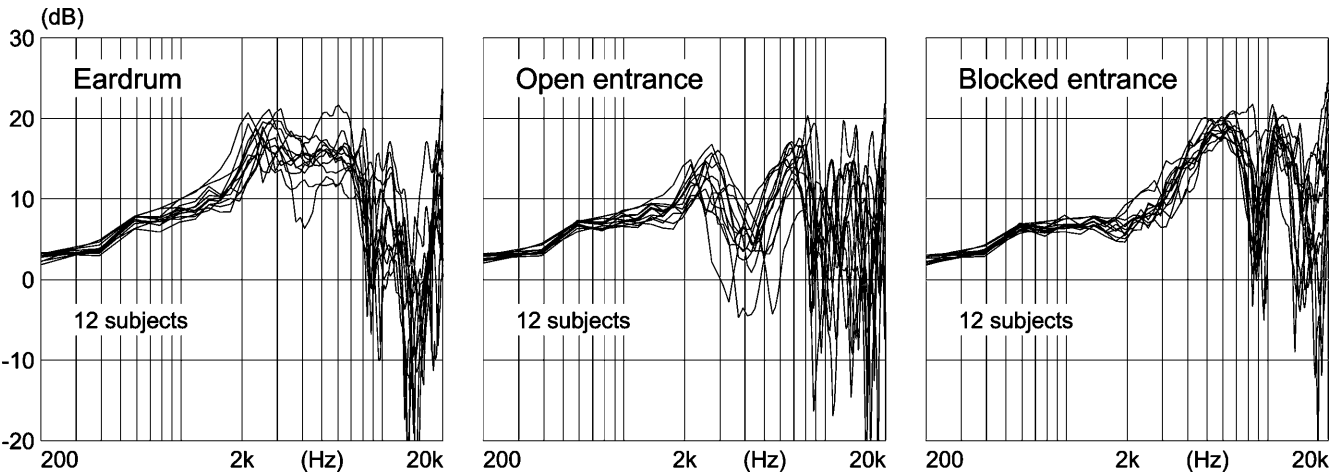
\includegraphics[scale=.25]{graph/OETF}
			%\end{figure}
			%}
			%
			%\only<3>{	excitation patterns
			%\begin{figure}
				%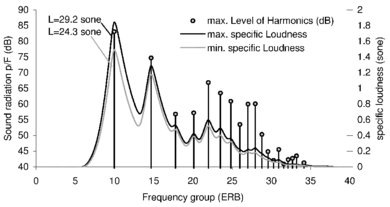
\includegraphics[scale=.5]{graph/excitationpatterns}
			%\end{figure}
			%}
			%\only<4>{	specific loudness
			%\begin{figure}
				%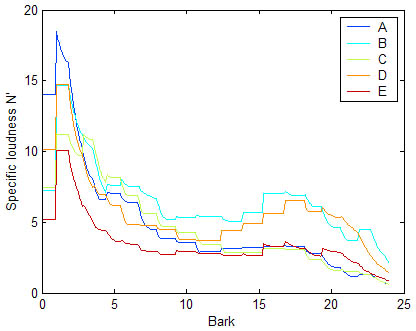
\includegraphics[scale=.4]{graph/specificloudness}
			%\end{figure}
			%}
		%\end{itemize}
        %\vspace{70mm}
		%}
	%\end{frame}
	        


    \section[summary]{lecture summary}
        \begin{frame}{summary}{lecture content}
            \begin{enumerate}
                \item   
                \smallskip
                \item<2->   
                \smallskip
                \item<3->   
                \smallskip
                \item<4->   
                \smallskip
                \item<5->   
            \end{enumerate}
        \end{frame}
\end{document}

